\documentclass[10pt]{beamer}
\usepackage{tikz}
\usepackage{pgfplots}
\usepackage{booktabs}
\usepackage{multirow}
\usepackage{array}
\usepackage{siunitx}
\usepackage{makecell}

\pgfplotsset{compat=newest}
\setbeamertemplate{navigation symbols}{}

% Add section pages
\AtBeginSection[]{
  \begin{frame}
    \vfill
    \centering
    \begin{beamercolorbox}[sep=8pt,center,shadow=true,rounded=true]{title}
    \usebeamerfont{title}\insertsectionhead\par%
    \end{beamercolorbox}
    \vfill
  \end{frame}
}

% Add page number to the lower right corner
\setbeamertemplate{footline}{%
  \hfill\usebeamercolor[fg]{page number in head/foot}%
  \usebeamerfont{page number in head/foot}%
  \insertframenumber\,/\,\inserttotalframenumber\hspace*{1ex}\vskip2pt%
}

% Customize the page number appearance
\setbeamercolor{page number in head/foot}{fg=gray}
\setbeamerfont{page number in head/foot}{size=\small}

\title{The Shell}
\author{Tzu-You Lin}
\setbeamerfont{title}{size=\huge}
\date{April 2, 2025}

\begin{document}

\begin{frame}
    \titlepage
\end{frame}

\begin{frame}
    \frametitle{Outline}
    \tableofcontents
\end{frame}

\section{Introduction}

\begin{frame}
    \frametitle{What is the Shell?}
    \begin{itemize}
        \item A command-line interface for interacting with the operating system
        \item Allows users to execute commands by typing them
        \item Provides a scripting environment for automating tasks
        \item Acts as an intermediary between the user and the system's kernel
    \end{itemize}
\end{frame}

\begin{frame}
    \frametitle{Shell Interface Examples}
    \begin{figure}
        \centering
        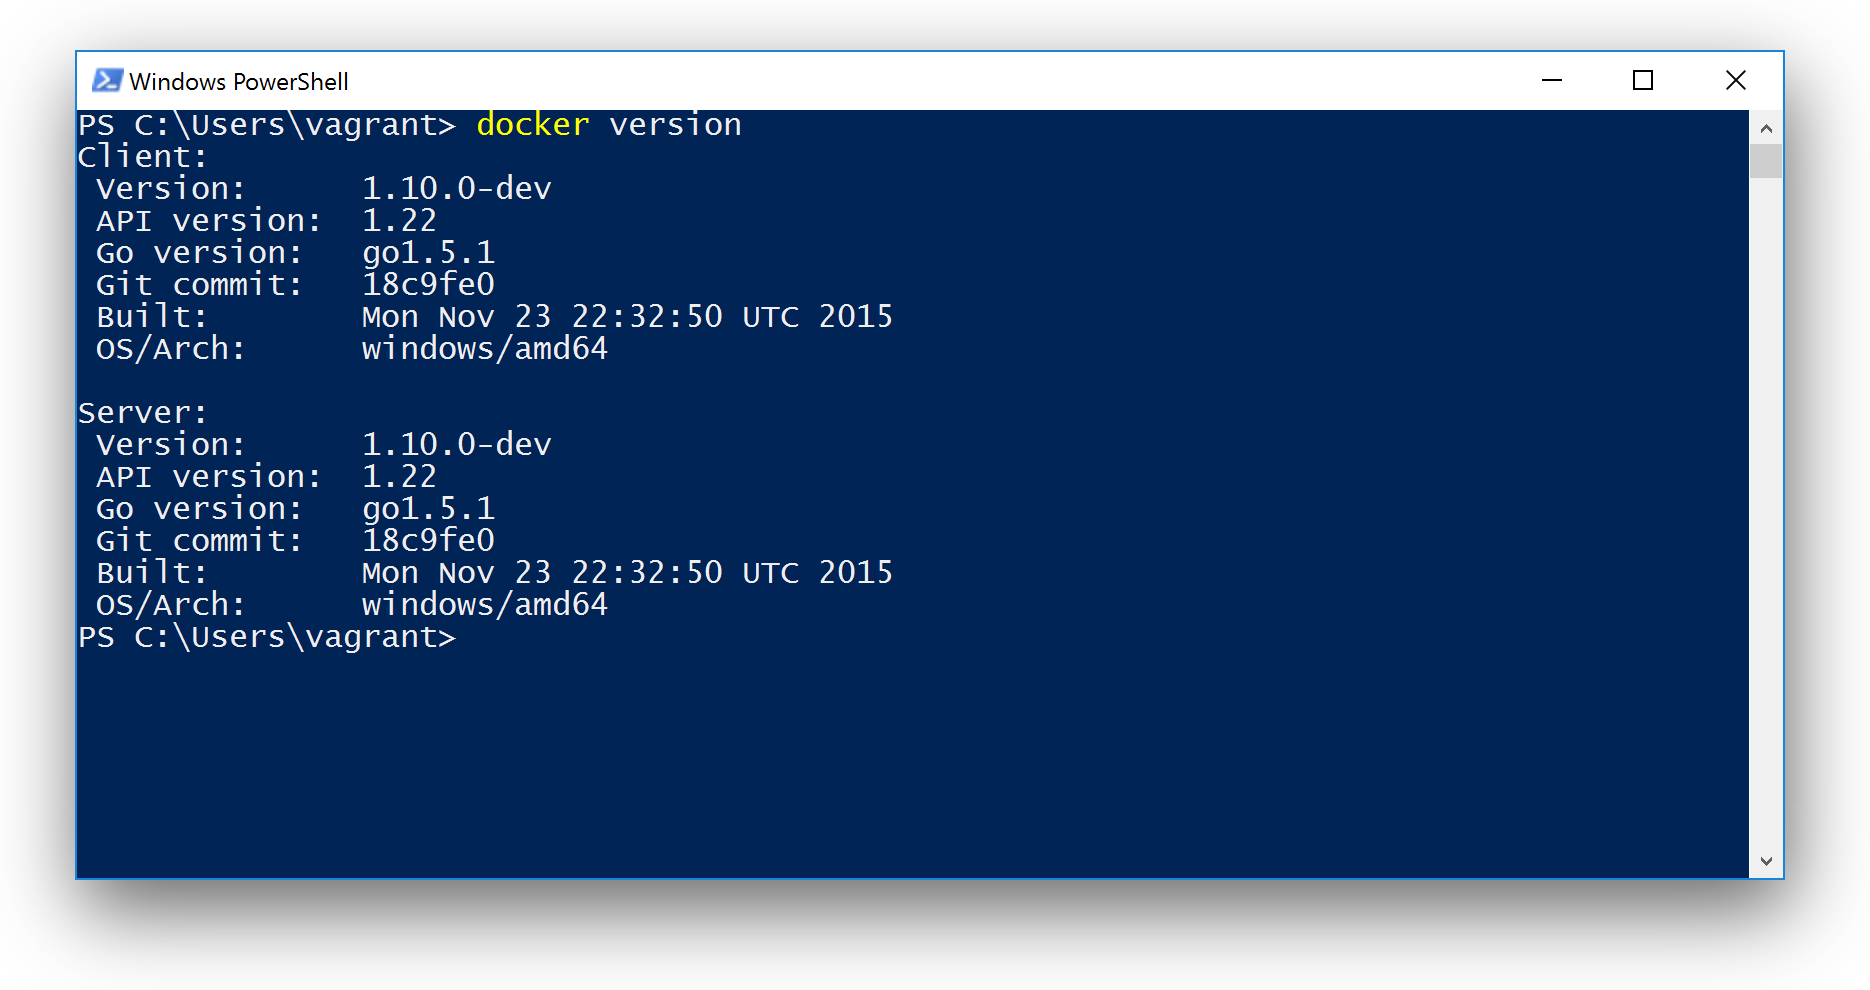
\includegraphics[width=0.8\textwidth]{images/windows.png}
        \caption{Windows PowerShell}
    \end{figure}
\end{frame}

\begin{frame}
    \frametitle{Shell Interface Examples (Cont.)}
    \begin{figure}
        \centering
        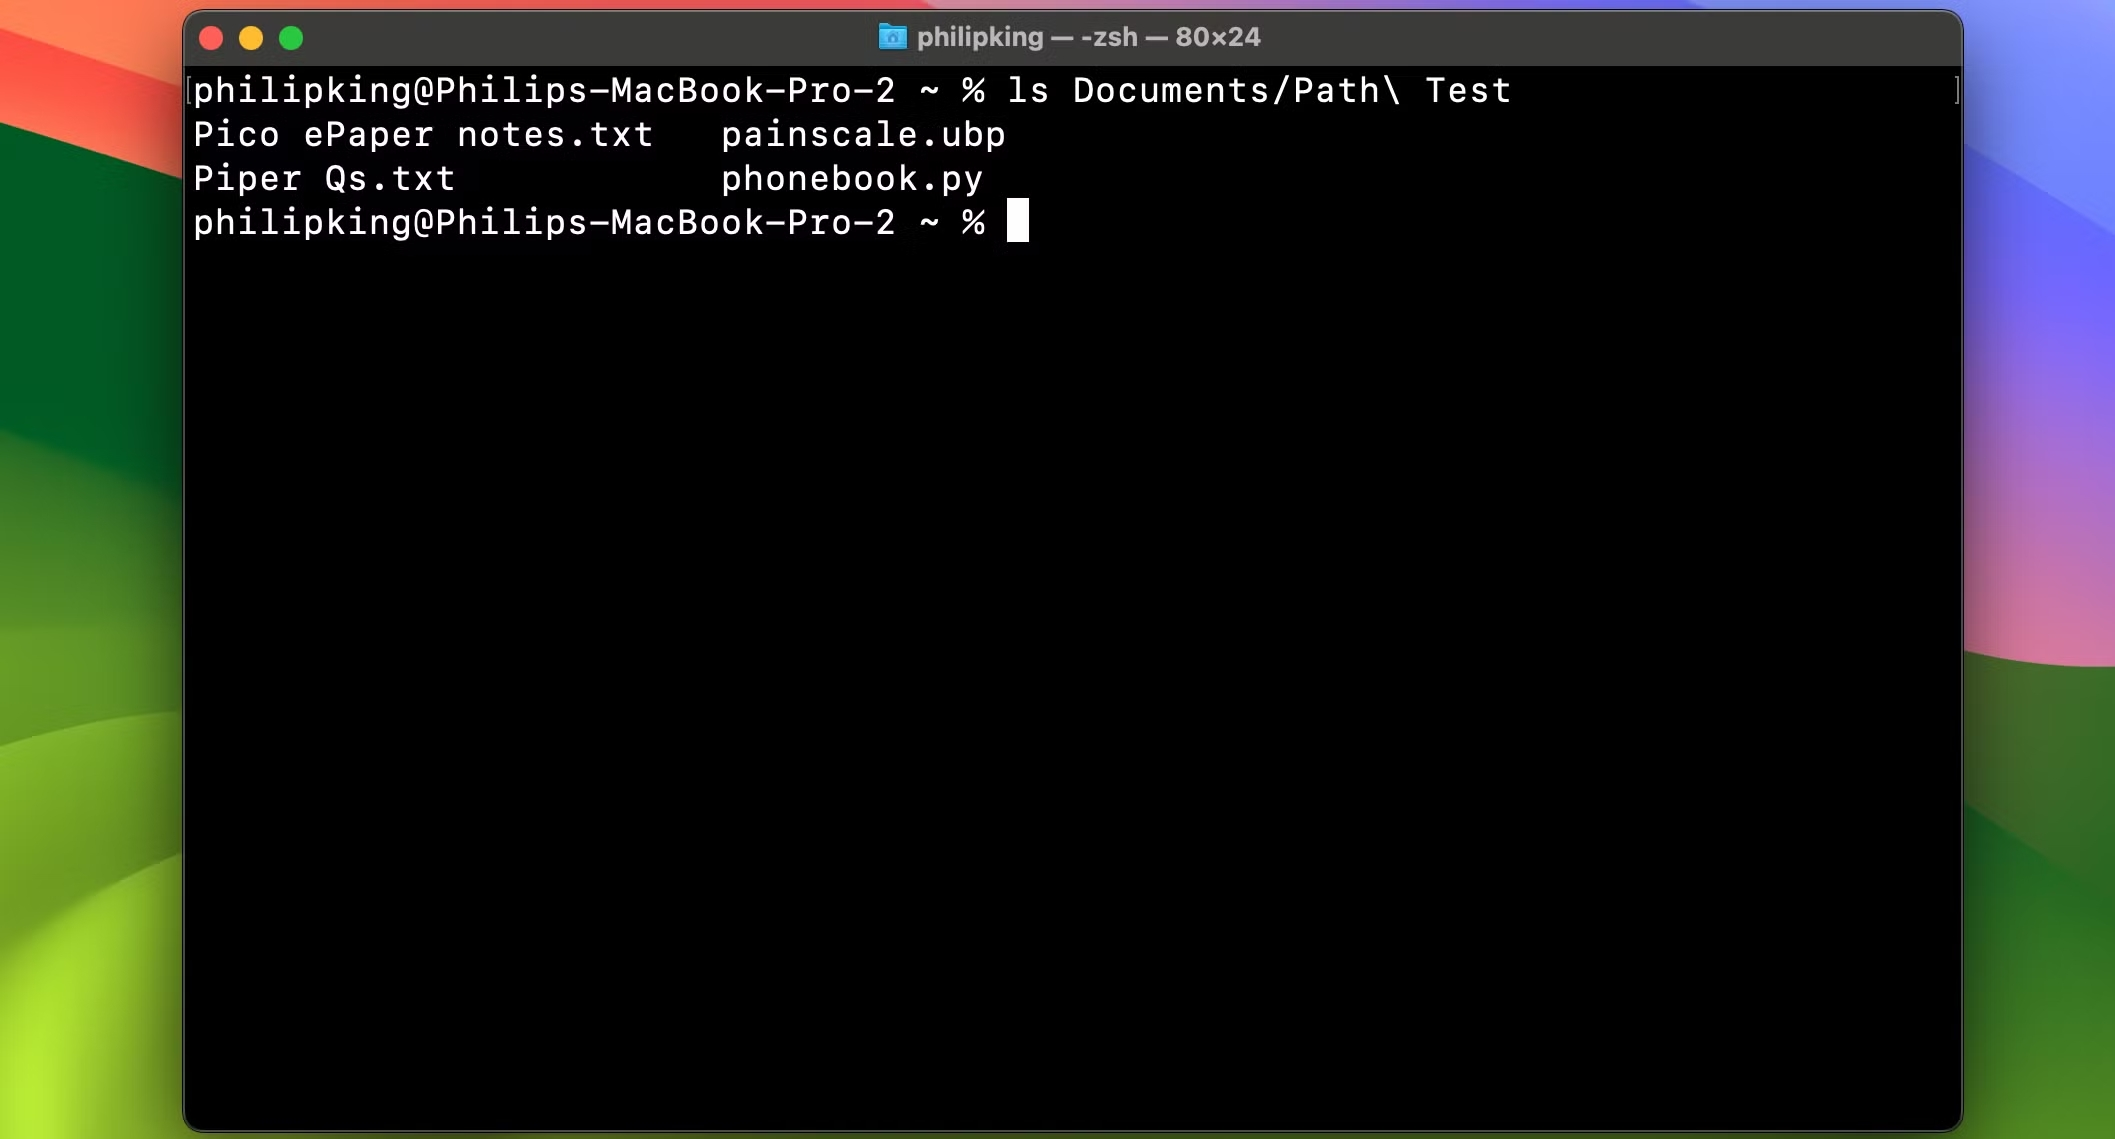
\includegraphics[width=0.8\textwidth]{images/macos.jpg}
        \caption{MacOS Terminal}
    \end{figure}
\end{frame}

\begin{frame}
    \frametitle{Shell Interface Examples (Cont.)}
    \begin{figure}
        \centering
        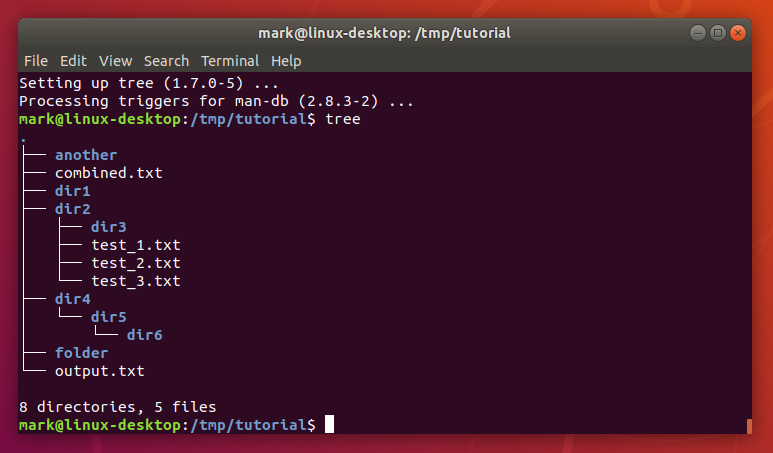
\includegraphics[width=0.8\textwidth]{images/linux.png}
        \caption{Linux Terminal}
    \end{figure}
\end{frame}

\begin{frame}
    \frametitle{Why Using The Shell?}
    \begin{itemize}
        \item Powerful command execution and problem-solving capabilities beyond what GUIs can offer
        \item Avoids memory complications associated with heavy applications and IDEs
        \item Efficient text-based interface for system interaction and file manipulation
        \item Automation and reproducibility through scripting, unlike manual GUI clicking
        \item Essential for high-performance computing and server administration
        \item Streamlines complex workflows by combining multiple programs and scripts (e.g., using Makefiles)
        \item Better visibility and control of system processes
    \end{itemize}
\end{frame}

\begin{frame}
    \frametitle{The Unix Philosophy}
    \begin{itemize}
        \item The shell tools we use today originate from the Unix family of operating systems
        \item Developed at Bell Labs in the 1970s
        \item Embodies the core Unix philosophy:
        \begin{quote}
            \textit{"Do One Thing And Do It Well"}
        \end{quote}
        \item Key principles:
        \begin{itemize}
            \item Pair and chain well-designed individual components
            \item Build powerful complex systems from simple parts
            \item Minimalist and modular approach
        \end{itemize}
        \item This philosophy is clearly reflected in Unix shell design and functionality
    \end{itemize}
\end{frame}

\begin{frame}
    \frametitle{Common Shell Use Cases}
    \begin{itemize}
        \item Version Control
        \begin{itemize}
            \item Managing code repositories with Git
            \item Tracking changes and collaborating on projects
            \item Branching and merging code
        \end{itemize}
        \item Development Tasks
        \begin{itemize}
            \item Compiling source code
            \item Running scripts and programs
            \item Managing build processes
        \end{itemize}
        \item File System Navigation
        \begin{itemize}
            \item Searching for files and directories
            \item Organizing and managing files
            \item Batch file operations
        \end{itemize}
        \item System Administration
        \begin{itemize}
            \item Monitoring system resources
            \item Managing processes
            \item Installing and updating software
        \end{itemize}
    \end{itemize}
\end{frame}

\begin{frame}
    \frametitle{Learning the Shell: It's Worth It!}
    \begin{itemize}
        \item Don't be intimidated by the command line interface
        \begin{itemize}
            \item Like any tool, it becomes natural with practice
            \item Most computer-savvy students adapt quickly
        \end{itemize}
        \item The learning curve pays off:
        \begin{itemize}
            \item Increased productivity
            \item Better understanding of your system
            \item More control over your computing environment
        \end{itemize}
        \item Personal experience as an instructor:
        \begin{itemize}
            \item Students who embrace the shell become more confident
            \item They often wonder how they worked without it before
            \item Many make it their preferred way of working
        \end{itemize}
        \item Recommendation: Start small, practice regularly, and build up your skills
    \end{itemize}
\end{frame}

\section{Shell Basics}

\begin{frame}
    \frametitle{Terminologies}
    \begin{itemize}
        \item The shell goes by many names: Shell, Terminal, TTY, Command Prompt, and Command Line Interface (CLI)
        \item All refer to the text-based interface for interacting with your computer
        \item In this course, we'll use \textcolor{blue}{Bash} (Bourne Again SHell):
        \begin{itemize}
            \item Default shell on most Linux distributions and macOS
            \item Industry standard for shell scripting
            \item Rich feature set and extensive documentation
        \end{itemize}
        \item For Windows users:
        \begin{itemize}
            \item Install Windows Subsystem for Linux (WSL)
            \item Provides a full Linux environment on Windows
            \item Enables native Bash usage without virtualization
        \end{itemize}
    \end{itemize}
\end{frame}

\begin{frame}[fragile]
    \frametitle{Shell Prompt}
    When you open a shell, you'll see something like:
\begin{verbatim}
username@hostname:~$
\end{verbatim}
    \begin{itemize}
        \item Let's break down each part:
        \begin{itemize}
            \item \colorbox{gray!20}{\texttt{username}} Your unique user identifier on the system
            \item \colorbox{gray!20}{\texttt{@hostname}} The name of the computer / server you're using
            \item \colorbox{gray!20}{\texttt{:{\textasciitilde}}} Your directory path (where \colorbox{gray!20}{\texttt{\textasciitilde}} signifies the user's home directory)
            \item \colorbox{gray!20}{\texttt{\$}} Indicates you're a regular user (vs. \colorbox{gray!20}{\texttt{\#}} for root/admin), and is the start of your command prompt.
        \end{itemize}
    \end{itemize}
\end{frame}

\begin{frame}[fragile]
    \frametitle{Command Syntax}
    All Bash commands follow a consistent pattern:
\begin{verbatim}
command option(s) argument(s)
\end{verbatim}
    \begin{itemize}
        \item \colorbox{gray!20}{\texttt{command}}: The program or action you want to run
        \item \colorbox{gray!20}{\texttt{option(s)}}: Modifies how the command behaves (usually starts with {-} or {-}{-})
        \item \colorbox{gray!20}{\texttt{argument(s)}}: What the command should act upon (files, directories, text, etc.)
    \end{itemize}
    
    Examples:
\begin{verbatim}
$ ls -lh ~/Documents/
$ sort -u myfile.txt
\end{verbatim}
\end{frame}

\begin{frame}[fragile]
    \frametitle{Command Syntax (Cont.)}
    Note:
    \begin{itemize}
        \item Options and arguments are optional:
        \begin{verbatim}
$ ls                  # No options or arguments
$ ls ~/Documents/     # Just an argument
$ ls -lh              # Just options
\end{verbatim}
        \item The command itself is mandatory - you must specify what you want to do
    \end{itemize}
\end{frame}

\begin{frame}[fragile]
    \frametitle{Getting Help with the man Command}
    The \texttt{man} (manual) command provides detailed documentation for commands:
\begin{verbatim}
$ man ls     # Shows manual for ls command
\end{verbatim}
    \begin{itemize}
        \item Manual pages contain:
        \begin{itemize}
            \item Command description and purpose
            \item Available options
            \item Basic examples
            \item Common use cases
        \end{itemize}
        \item Most commands have a manual page - if you're unsure how to use a command, try \texttt{man command}
    \end{itemize}
\end{frame}

\begin{frame}[fragile]
    \frametitle{Root Directory and Home Directory}
    Two important locations in the filesystem:
    \begin{itemize}
        \item Root Directory (\texttt{/}):
        \begin{itemize}
            \item The top-level directory in the filesystem
            \item All other directories and files are under root
            \item Absolute paths always start from root
\begin{verbatim}
$ ls /
bin    etc    lib    opt    sbin   tmp    var
dev    home   media  proc   sys    usr
\end{verbatim}
        \end{itemize}
        \item Home Directory (\texttt{\textasciitilde} or \texttt{/home/username}):
        \begin{itemize}
            \item Personal directory for each user
            \item Stores user-specific files and settings
            \item Default location when opening terminal
\begin{verbatim}
$ echo ~        # Shows home directory path
/home/username
$ cd ~          # Goes to home directory
\end{verbatim}
        \end{itemize}
    \end{itemize}
\end{frame}


\begin{frame}[fragile]
    \frametitle{The pwd Command - Print Working Directory}
    The \texttt{pwd} command shows your current location in the filesystem:
\begin{verbatim}
$ pwd
/home/username/Documents
\end{verbatim}
    \begin{itemize}
        \item \texttt{pwd} stands for "Print Working Directory"
        \item Shows the full path from root (/) to your current directory
        \item Useful when you need to:
        \begin{itemize}
            \item Confirm your location in the filesystem
            \item Get the absolute path of your current directory
            \item Debug navigation issues
        \end{itemize}
        \item No options are typically needed for basic usage
    \end{itemize}
\end{frame}

\begin{frame}[fragile]
    \frametitle{The cd Command - Change Directory}
    The \colorbox{gray!20}{\texttt{cd}} command allows you to navigate between directories:
\begin{verbatim}
$ cd Documents/     # Move into Documents directory
$ cd ..            # Move up one directory
$ cd ~             # Go to home directory
$ cd /             # Go to root directory
\end{verbatim}
    \begin{itemize}
        \item \colorbox{gray!20}{\texttt{cd}} stands for "Change Directory"
        \item Common navigation shortcuts:
        \begin{itemize}
            \item \colorbox{gray!20}{\texttt{.}} - Current directory
            \item \colorbox{gray!20}{\texttt{..}} - Parent directory
            \item \colorbox{gray!20}{\texttt{\textasciitilde}} - Home directory
            \item \colorbox{gray!20}{\texttt{/}} - Root directory
        \end{itemize}
        \item You can use absolute paths (from root) or relative paths:
\begin{verbatim}
$ cd /home/username/Documents    # Absolute path
$ cd ./projects                  # Relative path
\end{verbatim}
        \item If no path is specified, \colorbox{gray!20}{\texttt{cd}} defaults to home directory
    \end{itemize}
\end{frame}

\begin{frame}[fragile]
    \frametitle{Handling Spaces in File and Directory Names}
    \textbf{Problem:}
        
     Spaces in filenames create problems in the command line, since the shell treats each word separated by spaces as a different argument:
    \begin{verbatim}
$ cd My Documents     # ERROR: Shell sees two separate arguments
    \end{verbatim}
    \textbf{Solutions:}
    \begin{enumerate}
        \item Use quotes around the entire path:
\begin{verbatim}
$ cd "My Documents"   # Enclose path in quotes
\end{verbatim}
        \item Use escape characters (backslash) or tab completion:
\begin{verbatim}
$ cd My\ Documents    # Escape the space with backslash
$ cd My<TAB>         # Tab completion handles spaces
\end{verbatim}
        \item Best practice: Avoid using spaces in directory and file names
        \begin{itemize}
            \item Use underscores: \texttt{My\_Documents}
            \item Use hyphens: \texttt{My-Documents} 
            \item Use camelCase: \texttt{MyDocuments}
        \end{itemize}
    \end{enumerate}
\end{frame}

\begin{frame}[fragile]
    \frametitle{Listing Files and Directories with ls}
    
    \textbf{Basic Usage:}
    \begin{itemize}
        \item The \colorbox{gray!20}{\texttt{ls}} command lists files and directories
        \item Simple usage shows names only:
\begin{verbatim}
$ ls
Documents  Downloads  Pictures  test.txt
\end{verbatim}
    \end{itemize}

    \textbf{Detailed Information:}
    \begin{itemize}
        \item Use \colorbox{gray!20}{\texttt{ls -lh}} for detailed listing:
\begin{verbatim}
$ ls -lh
drwxr-xr-x 2 user group 4.0K Sep 20 10:30 Documents
-rw-r--r-- 1 user group  123B Sep 19 15:45 test.txt
\end{verbatim}
    \end{itemize}

    \textbf{Note:}
    \begin{itemize}
        \item The detailed listing shows permissions, owner, group, size, and timestamps
        \item For more information about file permissions and other details shown, we encourage you to search online
    \end{itemize}
\end{frame}

\begin{frame}[fragile]
    \frametitle{Creating Files with touch}
    
    \textbf{Basic Usage:}
    \begin{itemize}
        \item The \colorbox{gray!20}{\texttt{touch}} command creates empty files
        \item Example:
\begin{verbatim}
$ touch newfile.txt
$ ls
newfile.txt
\end{verbatim}
    \end{itemize}

    \textbf{Note:}
    \begin{itemize}
        \item Creates an empty file if it doesn't exist
        \item Updates timestamp if file already exists
    \end{itemize}
\end{frame}

\begin{frame}[fragile]
    \frametitle{Removing Files and Directories with rm}
    
    \textbf{Basic Usage:}
    \begin{itemize}
        \item The \colorbox{gray!20}{\texttt{rm}} command removes files
        \item Example:
\begin{verbatim}
$ rm oldfile.txt
$ ls
Documents  Downloads  Pictures
\end{verbatim}
    \end{itemize}

    \textbf{Removing Directories:}
    \begin{itemize}
        \item Use \colorbox{gray!20}{\texttt{rm -rf}} to remove directories and their contents
        \item Example:
\begin{verbatim}
$ rm -rf OldDirectory
$ ls
Documents  Pictures
\end{verbatim}
    \end{itemize}

    \textbf{Warning:}
    \begin{itemize}
        \item \textcolor{red}{Be extremely careful with \texttt{rm -rf}}
        \item Files and directories are permanently deleted
        \item No confirmation prompt and no recovery possible
        \item Double-check what you're deleting before pressing Enter
    \end{itemize}
\end{frame}

\begin{frame}[fragile]
    \frametitle{Moving Files with mv}
    
    \textbf{Basic Usage:}
    \begin{itemize}
        \item The \colorbox{gray!20}{\texttt{mv}} command moves or renames files
        \item Example of moving:
\begin{verbatim}
$ mv file.txt Documents/
$ ls Documents/
file.txt
\end{verbatim}
        \item Example of renaming:
\begin{verbatim}
$ mv oldname.txt newname.txt
$ ls
newname.txt
\end{verbatim}
    \end{itemize}

    \textbf{Note:}
    \begin{itemize}
        \item Will overwrite existing files without warning
        \item Use \texttt{mv -i} for interactive mode with prompts
        \item Can move multiple files to a directory at once
    \end{itemize}
\end{frame}

\begin{frame}[fragile]
    \frametitle{Copying Files with cp}
    
    \textbf{Basic Usage:}
    \begin{itemize}
        \item The \colorbox{gray!20}{\texttt{cp}} command copies files
        \item Example of copying a file:
\begin{verbatim}
$ cp source.txt backup.txt
$ ls
source.txt  backup.txt
\end{verbatim}
    \end{itemize}

    \textbf{Copying Directories:}
    \begin{itemize}
        \item Use \colorbox{gray!20}{\texttt{cp -r}} for directories
        \item Example:
\begin{verbatim}
$ cp -r Documents/ Backup/
$ ls
Documents/  Backup/
\end{verbatim}
    \end{itemize}

    \textbf{Note:}
    \begin{itemize}
        \item Will overwrite existing files without warning
        \item Use \texttt{cp -i} for interactive mode with prompts
        \item The \texttt{-p} flag preserves file permissions and timestamps
    \end{itemize}
\end{frame}

\begin{frame}[fragile]
    \frametitle{Further Exploration}
    
    \textbf{For More Advanced File Operations:}
    \begin{itemize}
        \item Learn about the powerful \colorbox{gray!20}{\texttt{find}} command for searching files
        \item Explore wildcards (*, ?, [...]) for pattern matching
        \item These tools will help you work more efficiently with files
    \end{itemize}

    \textbf{Example Topics to Look Up:}
    \begin{itemize}
        \item Finding files by name, type, or modification time
        \item Using wildcards with \texttt{cp}, \texttt{mv}, and other commands
        \item Combining commands for complex file operations
    \end{itemize}
\end{frame}

\section{File Processing}

\begin{frame}[fragile]
    \frametitle{Common Data File Formats}
    
    \textbf{Text-Based Formats:}
    \begin{itemize}
        \item \colorbox{gray!20}{\texttt{.csv}} (Comma-Separated Values)
        \begin{itemize}
            \item Simple, readable text format
            \item Each line is a record, fields separated by commas
            \item Universal support across platforms and tools
        \end{itemize}
        \item \colorbox{gray!20}{\texttt{.txt}} (Plain Text)
        \begin{itemize}
            \item Basic text data, often tab or space-delimited
            \item Easy to read and edit manually
        \end{itemize}
    \end{itemize}

    \textbf{Spreadsheet and Statistical Formats:}
    \begin{itemize}
        \item \colorbox{gray!20}{\texttt{.xlsx}} / \texttt{.xls} (Excel)
        \begin{itemize}
            \item Microsoft Excel's native format
            \item Supports multiple sheets, formulas, and formatting
        \end{itemize}
        \item \colorbox{gray!20}{\texttt{.dta}} (Stata)
        \begin{itemize}
            \item Native format for Stata statistical software
            \item Preserves variable labels and metadata
        \end{itemize}
        \item \colorbox{gray!20}{\texttt{.sav}} (SPSS)
        \begin{itemize}
            \item IBM SPSS Statistics format
            \item Includes variable and value labels
        \end{itemize}
    \end{itemize}
\end{frame}

\begin{frame}[fragile]
    \frametitle{Basic Text File Viewing Commands}
    
    \textbf{Common Commands for Viewing Text Files:}
    \begin{itemize}
        \item \colorbox{gray!20}{\texttt{cat}} (concatenate)
        \begin{itemize}
            \item Displays entire contents of file(s)
            \item Usage: \texttt{cat filename.txt}
            \item Can combine multiple files: \texttt{cat file1.txt file2.txt}
        \end{itemize}
        
        \item \colorbox{gray!20}{\texttt{head}} 
        \begin{itemize}
            \item Shows first few lines of a file
            \item Default: first 10 lines
            \item Specify lines: \texttt{head -n 5 filename.txt}
        \end{itemize}
        
        \item \colorbox{gray!20}{\texttt{tail}}
        \begin{itemize}
            \item Shows last few lines of a file
            \item Default: last 10 lines
            \item Follow updates: \texttt{tail -f logfile.txt}
            \item Specify lines: \texttt{tail -n 20 filename.txt}
        \end{itemize}
    \end{itemize}
\end{frame}

\begin{frame}[fragile]
    \frametitle{Advanced Text Processing Commands}
    
    \textbf{Powerful Text Processing Tools:}
    \begin{itemize}
        \item \colorbox{gray!20}{\texttt{grep}} (Global Regular Expression Print)
        \begin{itemize}
            \item Searches text patterns in files
            \item Usage: \texttt{grep "pattern" filename.txt}
            \item Supports regular expressions for complex searches
        \end{itemize}
        
        \item \colorbox{gray!20}{\texttt{sed}} (Stream Editor)
        \begin{itemize}
            \item Performs text transformations on input
            \item Common for search and replace operations
            \item Example: \texttt{sed 's/old/new/g' filename.txt}
        \end{itemize}
        
        \item \colorbox{gray!20}{\texttt{awk}}
        \begin{itemize}
            \item Powerful text processing programming language
            \item Excellent for column-based data processing
            \item Can perform calculations and complex text operations
        \end{itemize}
    \end{itemize}
    
    \vspace{0.5em}
    \textbf{Note:} These are advanced tools that require significant practice to master.
\end{frame}

\section{Programming}

\begin{frame}[fragile]
    \frametitle{Running Python Scripts}
    \begin{itemize}
        \item Python scripts can be run directly from the shell
        \item Basic syntax: \colorbox{gray!20}{\texttt{python script.py}}
        \item Common variations:
        \begin{itemize}
            \item Python version specific: \colorbox{gray!20}{\texttt{python3 script.py}}
        \end{itemize}
    \end{itemize}
\end{frame}

\begin{frame}[fragile]
    \frametitle{Running R Scripts}
    \begin{itemize}
        \item R scripts can be executed from the command line using Rscript
        \item Basic syntax: \colorbox{gray!20}{\texttt{Rscript script.R}}
        \item Common variations:
        \begin{itemize}
            \item Execute R commands directly: \colorbox{gray!20}{\texttt{Rscript -e "print('Hello')"}}
        \end{itemize}
        \item Alternative: Using R interpreter
        \begin{itemize}
            \item Start R console: \colorbox{gray!20}{\texttt{R}}
            \item Source script: \colorbox{gray!20}{\texttt{source("script.R")}}
        \end{itemize}
    \end{itemize}
\end{frame}

\begin{frame}[fragile]
    \frametitle{Understanding Redirection}
    \begin{itemize}
        \item Shell redirection allows you to control input/output streams
        \item Basic redirection operators:
        \begin{itemize}
            \item \colorbox{gray!20}{\texttt{>}} - Redirect output to a file (overwrite)
            \item \colorbox{gray!20}{\texttt{>>}} - Append output to a file
            \item \colorbox{gray!20}{\texttt{<}} - Take input from a file
        \end{itemize}
        \item Examples:
        \begin{itemize}
            \item Save command output: \colorbox{gray!20}{\texttt{ls -l > files.txt}}
            \item Append to log: \colorbox{gray!20}{\texttt{echo "Done" >> log.txt}}
        \end{itemize}
    \end{itemize}
\end{frame}


\begin{frame}[fragile]
    \frametitle{Input/Output Redirection with Scripts}
    \begin{itemize}
        \item Scripts can read input and write output to files using redirection
        \item Example Python script (\texttt{count.py}):
        \begin{itemize}
            \item \colorbox{gray!20}{\texttt{for line in sys.stdin: print(len(line))}}
            \item Reads each line and outputs its length
        \end{itemize}
        \item Running with redirection:
        \begin{itemize}
            \item Input from file: \colorbox{gray!20}{\texttt{python count.py < input.txt}}
            \item Output to file: \colorbox{gray!20}{\texttt{python count.py < input.txt > lengths.txt}}
            \item Append output: \colorbox{gray!20}{\texttt{python count.py < input.txt >> lengths.txt}}
        \end{itemize}
    \end{itemize}
\end{frame}

\begin{frame}[fragile]
    \frametitle{Automating Testing with Redirection and Diff}
    \begin{itemize}
        \item In this course, we encourage you to:
        \begin{itemize}
            \item Write Python programs that read from stdin and write to stdout
            \item Automate testing using input/output redirection
            \item Use \texttt{diff} to compare expected and actual outputs
        \end{itemize}
        \item Example testing workflow:
        \begin{itemize}
            \item Run program: \colorbox{gray!20}{\texttt{python main.py < test\_input.txt > actual\_output.txt}}
            \item Compare outputs: \colorbox{gray!20}{\texttt{diff expected\_output.txt actual\_output.txt}}
            \item No output from diff means outputs match exactly
        \end{itemize}
    \end{itemize}
\end{frame}


\begin{frame}
    \frametitle{References}

    \begin{itemize}
        \item These slides are adapted from:
        \begin{itemize}
            \item Grant McDermott's Data Science for Economists course materials
            \item \url{https://github.com/uo-ec607/lectures}
        \end{itemize}
    \end{itemize}
\end{frame}

\end{document}